%% {\it\color{red} Section Editors: Markus, Ed, Peter L.}
\label{sec:reco}

Dealing with the increased event complexity from unprecedented levels of pile-up, reaching an average of 140 simultaneous proton-proton collision ($\langle\mu\rangle$) during Run~4 and up to 200 in the subsequent Runs, poses a challenge in particular to the offline event reconstruction and to the physics object identification. At the same time, it will be vital for the ATLAS Phase-2 programme that the physics performance of the reconstructed objects will be preserved wherever possible improved w.r.t. the Run~2/3, despite the increasing level of pile-up expected for Phase-2.
%
\begin{table}[htb!]
  \caption{The CPU required in HS06~$\times$~seconds to reconstruct data 2018 events at an average of 90 pile-up from a dedicated high pile-up run when using the current software reconstruction software. Compared are the results for track reconstruction, muon and calorimeter reconstruction, combined reconstruction and monitoring using the Run~2 software release.}
  \label{tab:RecoCPU}
  \centering
  \begin{tabular}{|c|c||c|c|c|c||c|} \hline
    Detector & $\langle\mu\rangle$ & inner    & muon spectrometer & combined       & monitoring & total \\
             &                     & tracking & and calorimeter   & reconstruction &           &        \\ \hline
    %% old data 17: Run~2    & 50                  & 337      & 31                 & 24            & 25        & 29   & 462  \\ \hline
    %% master nightly Feb.2 on data 18 Raw to all, HS06 scaling of the machine is 22.
    Run~2    & 90                  & 1137     & 149               & 301            & 106       & 1693  \\ \hline
    %% Phase-2  & 140                 & 124      &                   &                &           &       \\
    %%          & 200                 & 214      &                   &                &           &       \\ \hline
    \end{tabular}
\end{table}

Estimates based using the current Run~2 software to reconstruct raw data from a dedicated run taken in 2018 with an average pile-up of 90, as shown in Table~\ref{tab:RecoCPU}, indicate that for the current detector and software all aspects of event reconstruction require significant CPU resources to deal with the increased event complexity, with the inner track reconstruction dominating in CPU needed because of its pronounced scaling with pile-up. ATLAS is undertaking a major detector and software upgrade program to facilitate the required physics performance improvements and at the same time to help reduce the CPU requirements for event reconstruction:
%
\begin{itemize}
    \item 
    The design of the Phase-2 tracker upgrade (ITk)~\cite{ATL-PHYS-PUB-2019-014} has been optimised not only for physics performance, but at the same time the design aims to minimise CPU for reconstruction at an average of 200 pile-up. The five layer ITk Pixel Detector with its ring design will facilitate fast track seeding and finding approaches.
    \item
    ATLAS carried out a prototype study~\cite{ATL-PHYS-PUB-2019-041} to demonstrate that classical CPU based algorithmic approaches can exploit the ITk detector design for a fast track reconstruction to resolve the CPU problem, at the expense of some limited loss in physics performance.
    \item
    ATLAS initiated the ACTS~\cite{acts} open source project to develop the next generation tracking software in a common cross experiment project, with the aim to use ACTS to achieve both, CPU reduction and excellent physics performance, for the Phase-2 reconstruction. Moving to ACTS will not only address the challenge of ITk reconstruction, but at the same time it will help reducing the CPU for other aspects of reconstruction, like particle flow or muon reconstruction.
    \item
    An equally important aspect of the ATLAS Phase-2 reconstruction strategy is a strong programme of algorithm R\&D to improve all aspects of event reconstruction, to further reduce the CPU needs and to maximise physics performance. This includes a broad set of R\&D initiatives of applying Machine Learning and novel data science inspired algorithmic approaches to reconstruction, as well as R\&D on exploiting co-processors (i.e. GPUs) for offline event reconstruction. 
\end{itemize}

%%%%%%%%%%%%%%%%%%%%%%%%%%%%%%%%%%%%%%%%%%%%%%%%%%%%%%%%%%%%%%%%%%%%%%%

\subsection{The Tracker Upgrade and the Fast Track Reconstruction Strategy for Phase-2}
\label{sub:ITKFastTrack}

%
\begin{figure}[htb!]
  \centering
  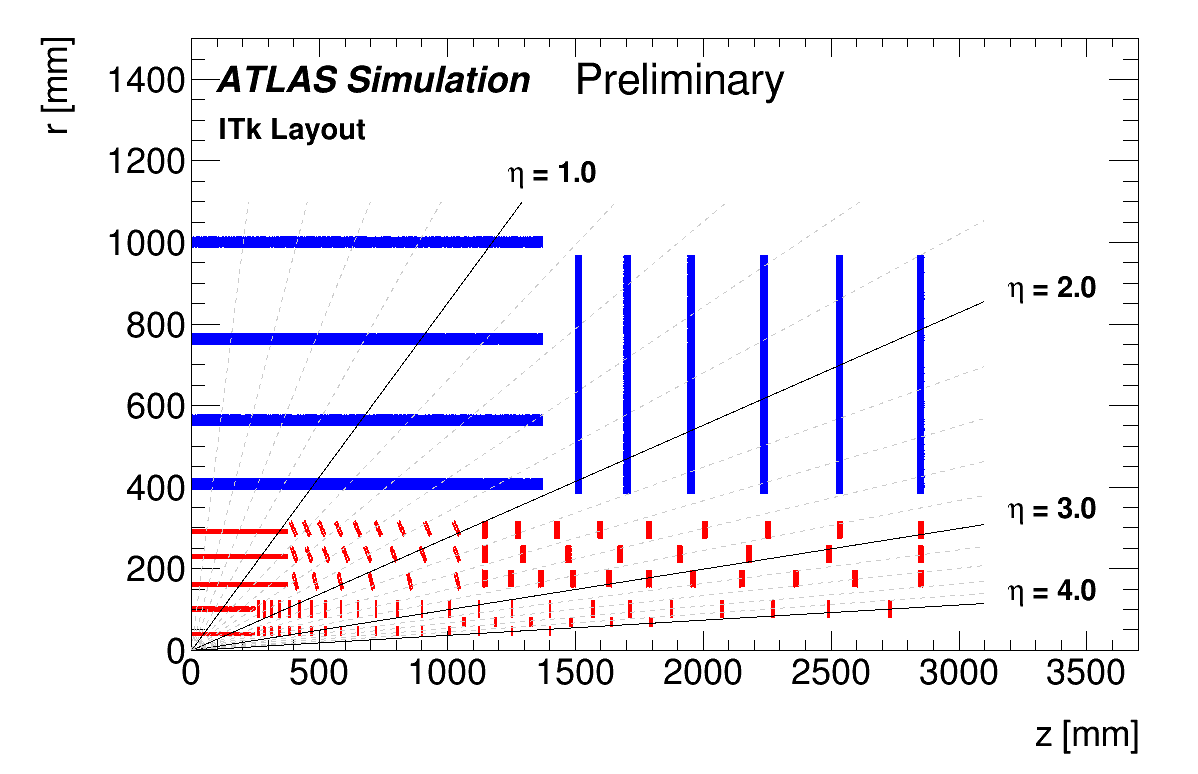
\includegraphics[width=0.51\textwidth]{figures/HitsRZ_Half_ITkLayout}
   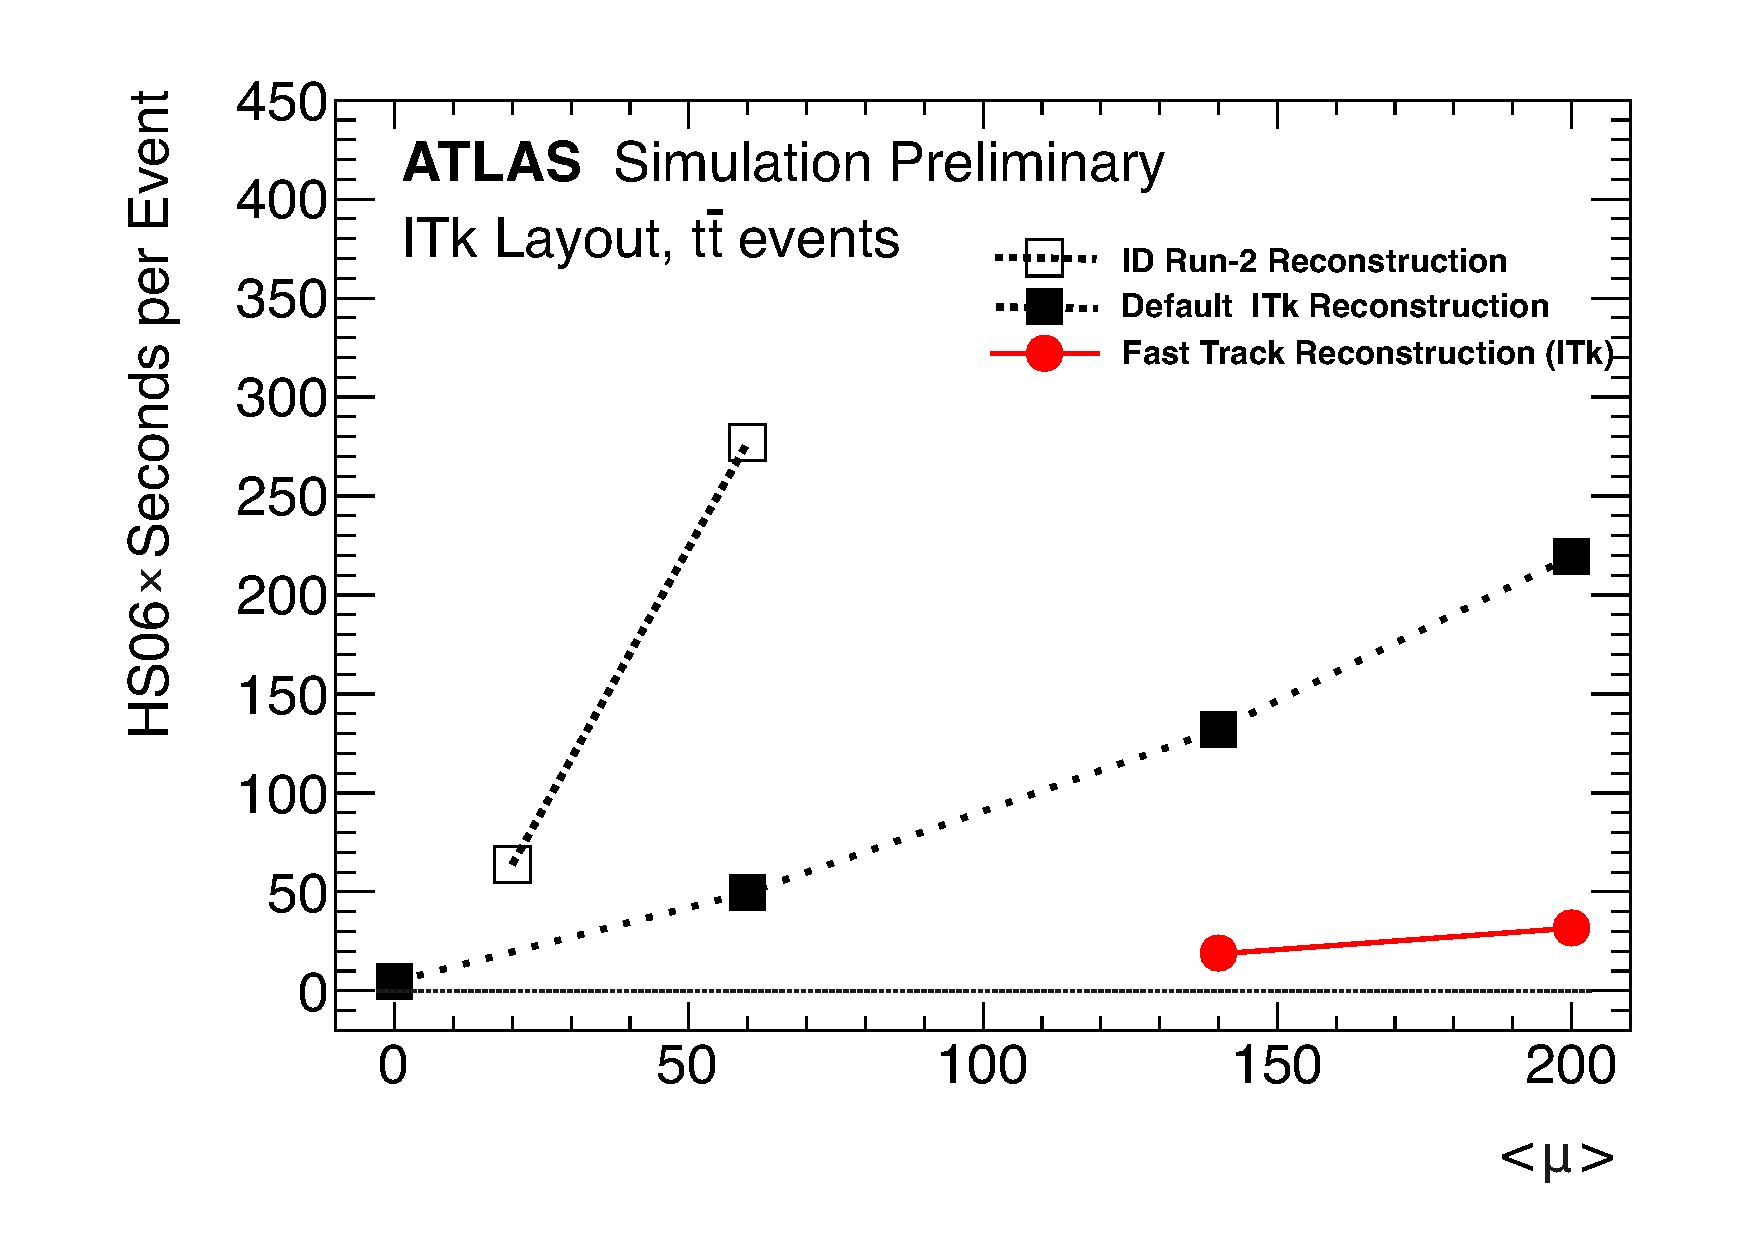
\includegraphics[width=0.47\textwidth]{figures/Timing_fast_ITkLayout_Run2}
  %% 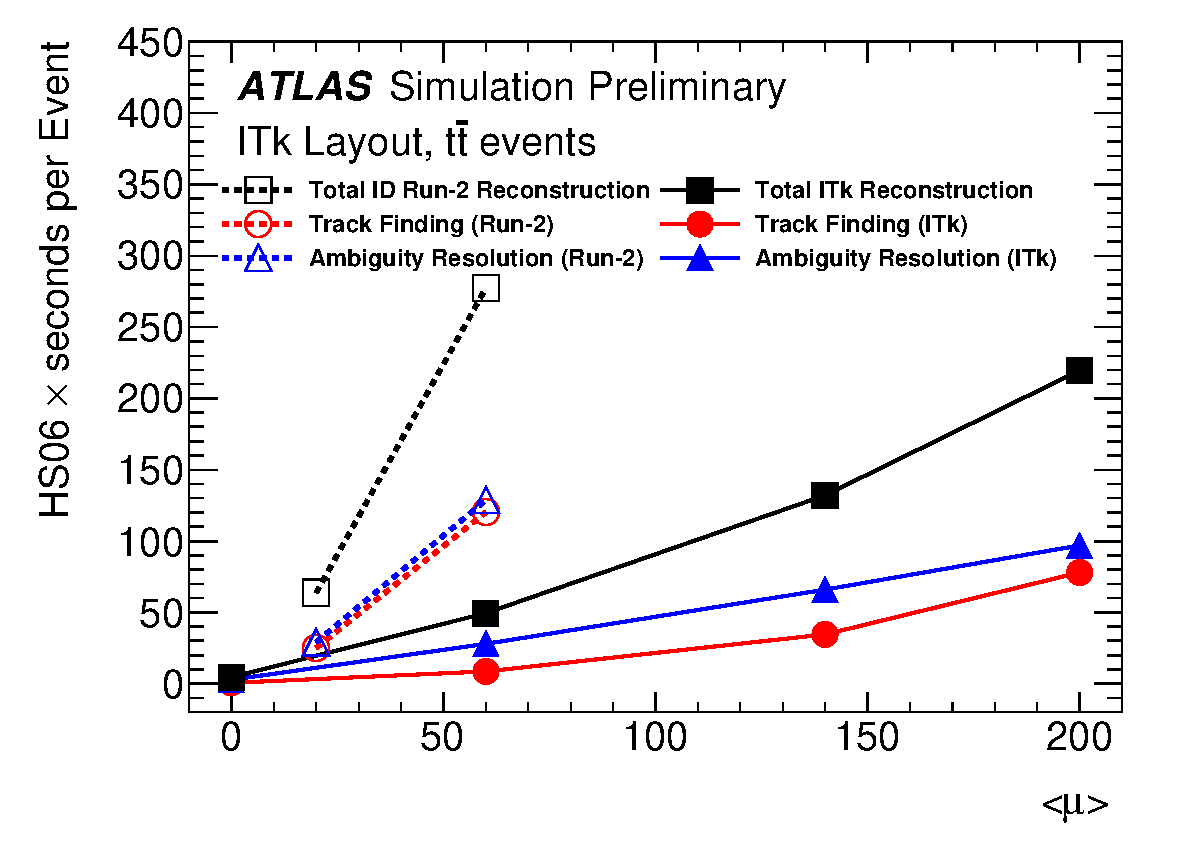
\includegraphics[width=0.47\textwidth]{figures/Timing_ITkLayout_Run2}
  \caption{{\bf Left:} A schematic layout of the ``ITk Layout'' with a five layer Pixel Detector (red) surrounded by the Strip Detector (blue). Only the positions of the active sensors are shown. {\bf Right:} The CPU required in HS06~$\times$~seconds to reconstruct a $t\bar{t}$~event in the current ID and the ITk at different levels of $\langle\mu\rangle$. Standard Run~2 reconstruction was used for the current ID, while for the ITk results are shown using the Run~2 software (black line) and the fast track reconstruction (red). Figures taken from References~\cite{ATL-PHYS-PUB-2019-014} and \cite{ATL-PHYS-PUB-2019-041}.}
  \label{fig:ITkandCPU}
\end{figure}

Figure~\ref{fig:ITkandCPU} illustrates the design of the ITk and the results of the fast track reconstruction study. The left plot shows a schematic $R-z$ view of the ITk detector layout that will consist of a five layer pixel system covering 8 units in $\eta$, surrounded by a four layer double sided strip detector with small stereo angle. The new tracking detector has been optimised for 200 pile-up, with an improved granularity, a constant hit coverage, a reduced material budget in the active tracking volume and a sensor placement that also aimed at minimising CPU for pattern recognition. The right plot shows the CPU required for track reconstruction as a function of average pile-up for the current ID and the ITk. Using the Run~2 tracking software to reconstruct the current ID, a strong scaling in CPU is observed between $\langle\mu\rangle = 20$ and $60$. Shown on the same plot is the CPU required by the Run~2 tracking code to reconstruct the ITk with an average event pile-up of up to 200. The ITk allows to significantly reduce the CPU to 124 and 214 HS06~$\times$~seconds, respectively, for an average pile-up of 140 and 200. At the same time the ITk will improve in physics performance compared to the current ID~\cite{ATL-PHYS-PUB-2019-014}.
%
\begin{table}[htb!]
  \caption{The CPU required in HS06~$\times$~seconds to reconstruct $t\bar{t}$ Monte Carlo events with $\langle\mu\rangle = 140$ and 200 in the ITk. Listed are the results for the different reconstruction steps using the current Run~2 software and the fast ITk track reconstruction. An Intel Xeon E5-2620v2 was used with 2.1~GHz and six physical cores per CPU. The CPU time is multiplied with the HS06 factor of 17.8 for single thread running. The Table is taken from Reference ~\cite{ATL-PHYS-PUB-2019-041}.}
  \label{tab:FastTrackCPU}
  \centering
  \begin{tabular}{|c|c||c|c|c|c|c||c|} \hline
   $\langle\mu\rangle$  & Tracking & Byte Stream                  & Cluster     & Space  & Si Track & Ambiguity  & Total \\
                        &          & Decoding                     & Finding     & Points & Finding  & Resolution & ITk   \\ \hline
   \multirow{2}{*}{140} &  Run~2   & \multirow{2}{*}{1.2$^{(*)}$}  & 17.1        & 6.0    & 41.1     &  58.2      & 124 \\
                        &  fast    &                              & 4.5         & 0.9    & 12.4     &  -         &  19.0 \\ \hline
   \multirow{2}{*}{200} &  Run~2   &  \multirow{2}{*}{1.6$^{(*)}$} & 26.3        & 8.6    & 85.8     &  92.0      & 214 \\
                        &  fast    &                              & 6.3         & 1.2    & 22.6     &  -         &  31.7 \\ \hline
  \end{tabular} \\
  $^{(*)}$ {\tiny Scaled from Run-2, see text.}
\end{table}

ATLAS has undertaken a study~\cite{ATL-PHYS-PUB-2019-041} to demonstrate the possible CPU performance improvements achievable by optimising the Run~2 track reconstruction techniques for Phase-2 levels of pile-up. The two tracking algorithms requiring the largest fraction of CPU are the Silicon Track Finding and the Ambiguity Resolution. The Ambiguity Resolution takes about 60\% of the total CPU time to apply the final precise track fit and to handle the pixel cluster splitting in dense environments using a Neural Network~\cite{Aad:2014yva}. For the purpose of this prototype study, the Ambiguity Resolution algorithm is omitted from the reconstruction chain. Instead, a tighter track selection and precise cluster calibrations are applied already at the stage of the Silicon Track Finding to remove duplicate tracks and fakes.
% The Silicon Track Finding algorithm now also makes use of the precise cluster calibrations, while still using an approximate material model and approximations in the cluster corrections.
The five layer Pixel Detector covers the full range of $|\eta| < 4$ such that the seed finding could rely only on pixel hit combinations, leaving out the strip seed iteration.
% For the purpose of this study the option for the recovery for Bremsstrahlung was temporarily disabled in the Silicon Track Finding.
In addition, technical improvements were applied e.g. to the strip and pixel clustering and space point formation to better optimise the software for Phase-2 levels of pile-up.

Table~\ref{tab:FastTrackCPU} summarises the CPU times for using both the Run~2 and the fast tracking code reconstruction for reconstructing the ITk. The fast version of Silicon Track Finding is approximately eight times faster for $\langle\mu\rangle = 140$ and 200, respectively. The fast track finding is about a factor 1.8 faster for the $\langle\mu\rangle = 140$ sample, compared to the $\langle\mu\rangle = 200$ sample. Adding the CPU needs for the Cluster Finding and the Space Point Finding algorithms, the total CPU requirement for the fast ITk track reconstruction becomes 19 and 31.7 HS06~$\times$~seconds for $\langle\mu\rangle = 140$ and 200, respectively. The left plot of Figure~\ref{fig:ITkandCPU} shows the result for the fast reconstruction in red.
%
\begin{figure}[htb!]
  \centering
  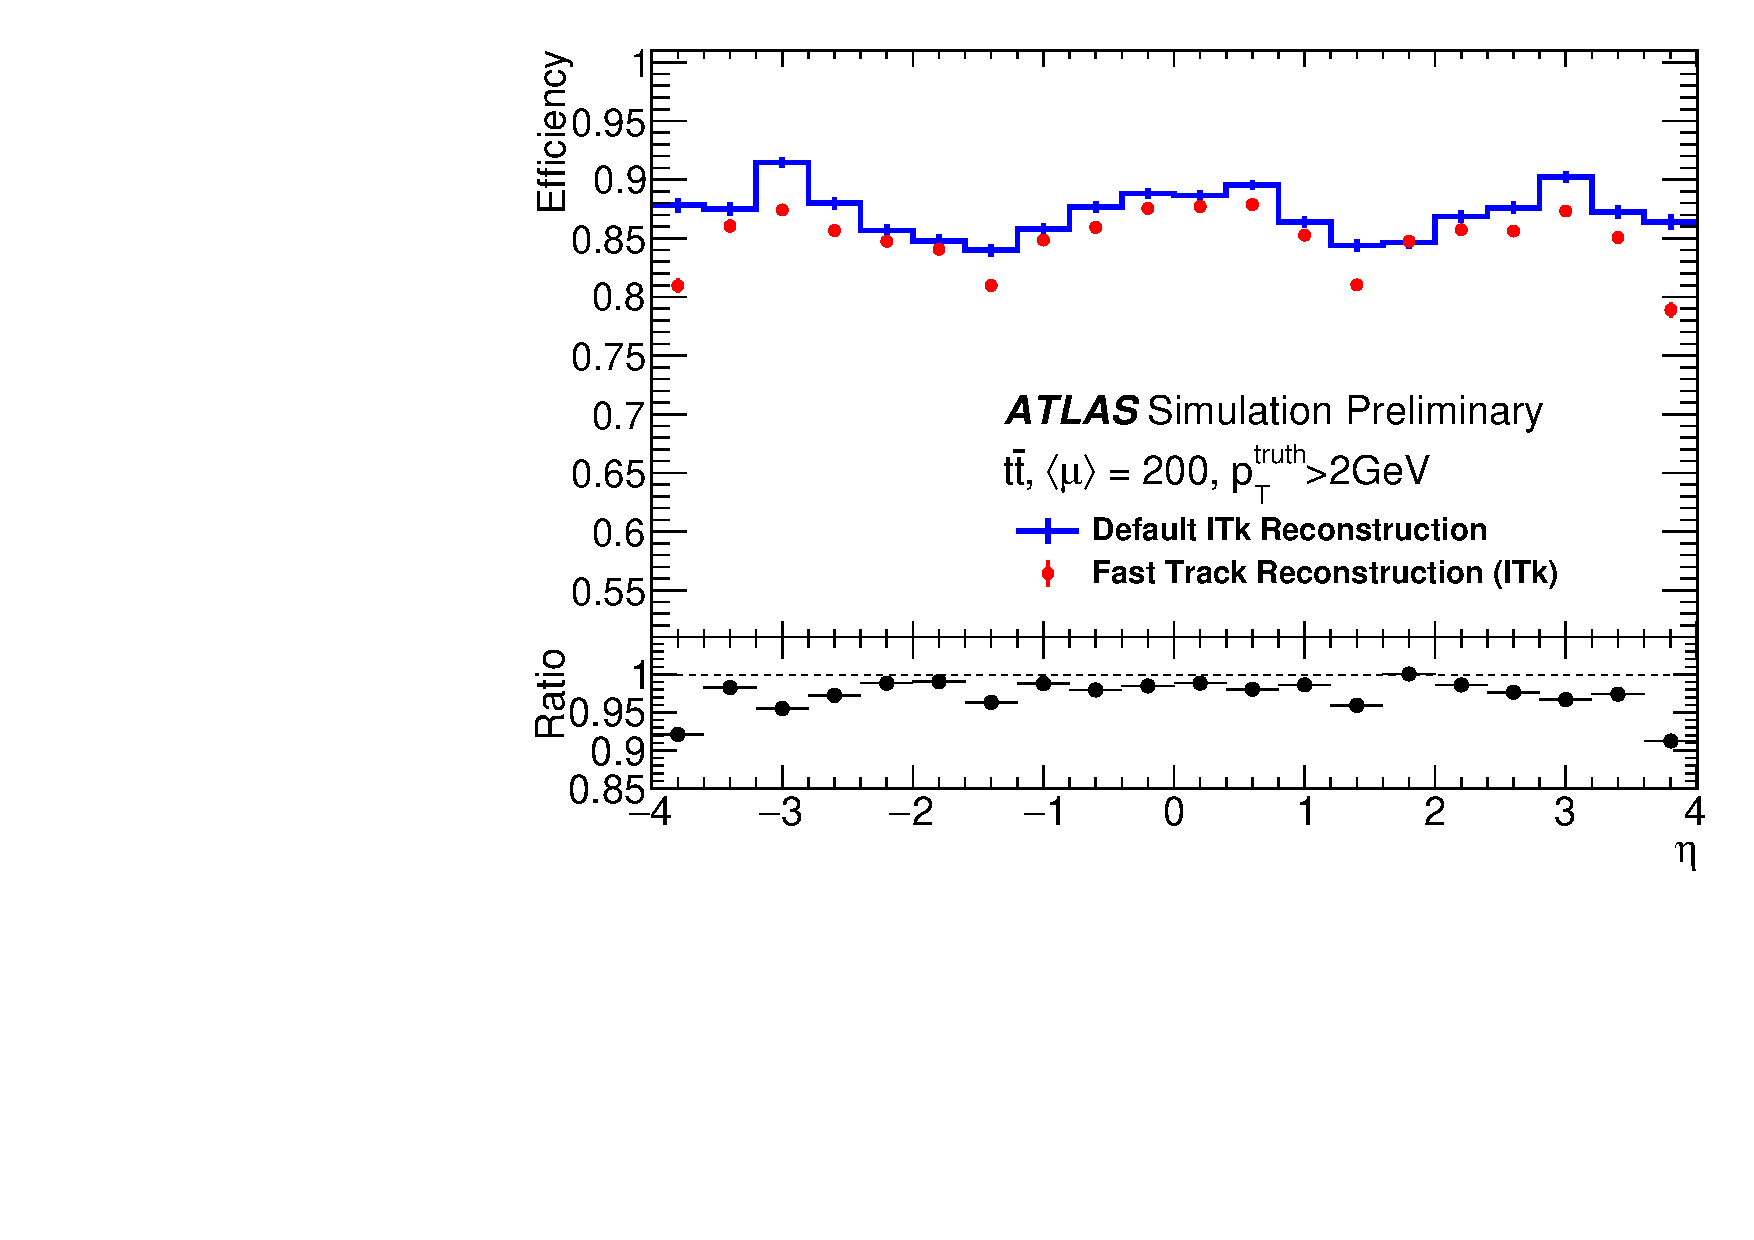
\includegraphics[width=0.48\textwidth]{figures/efficiencyEtaCombined}
  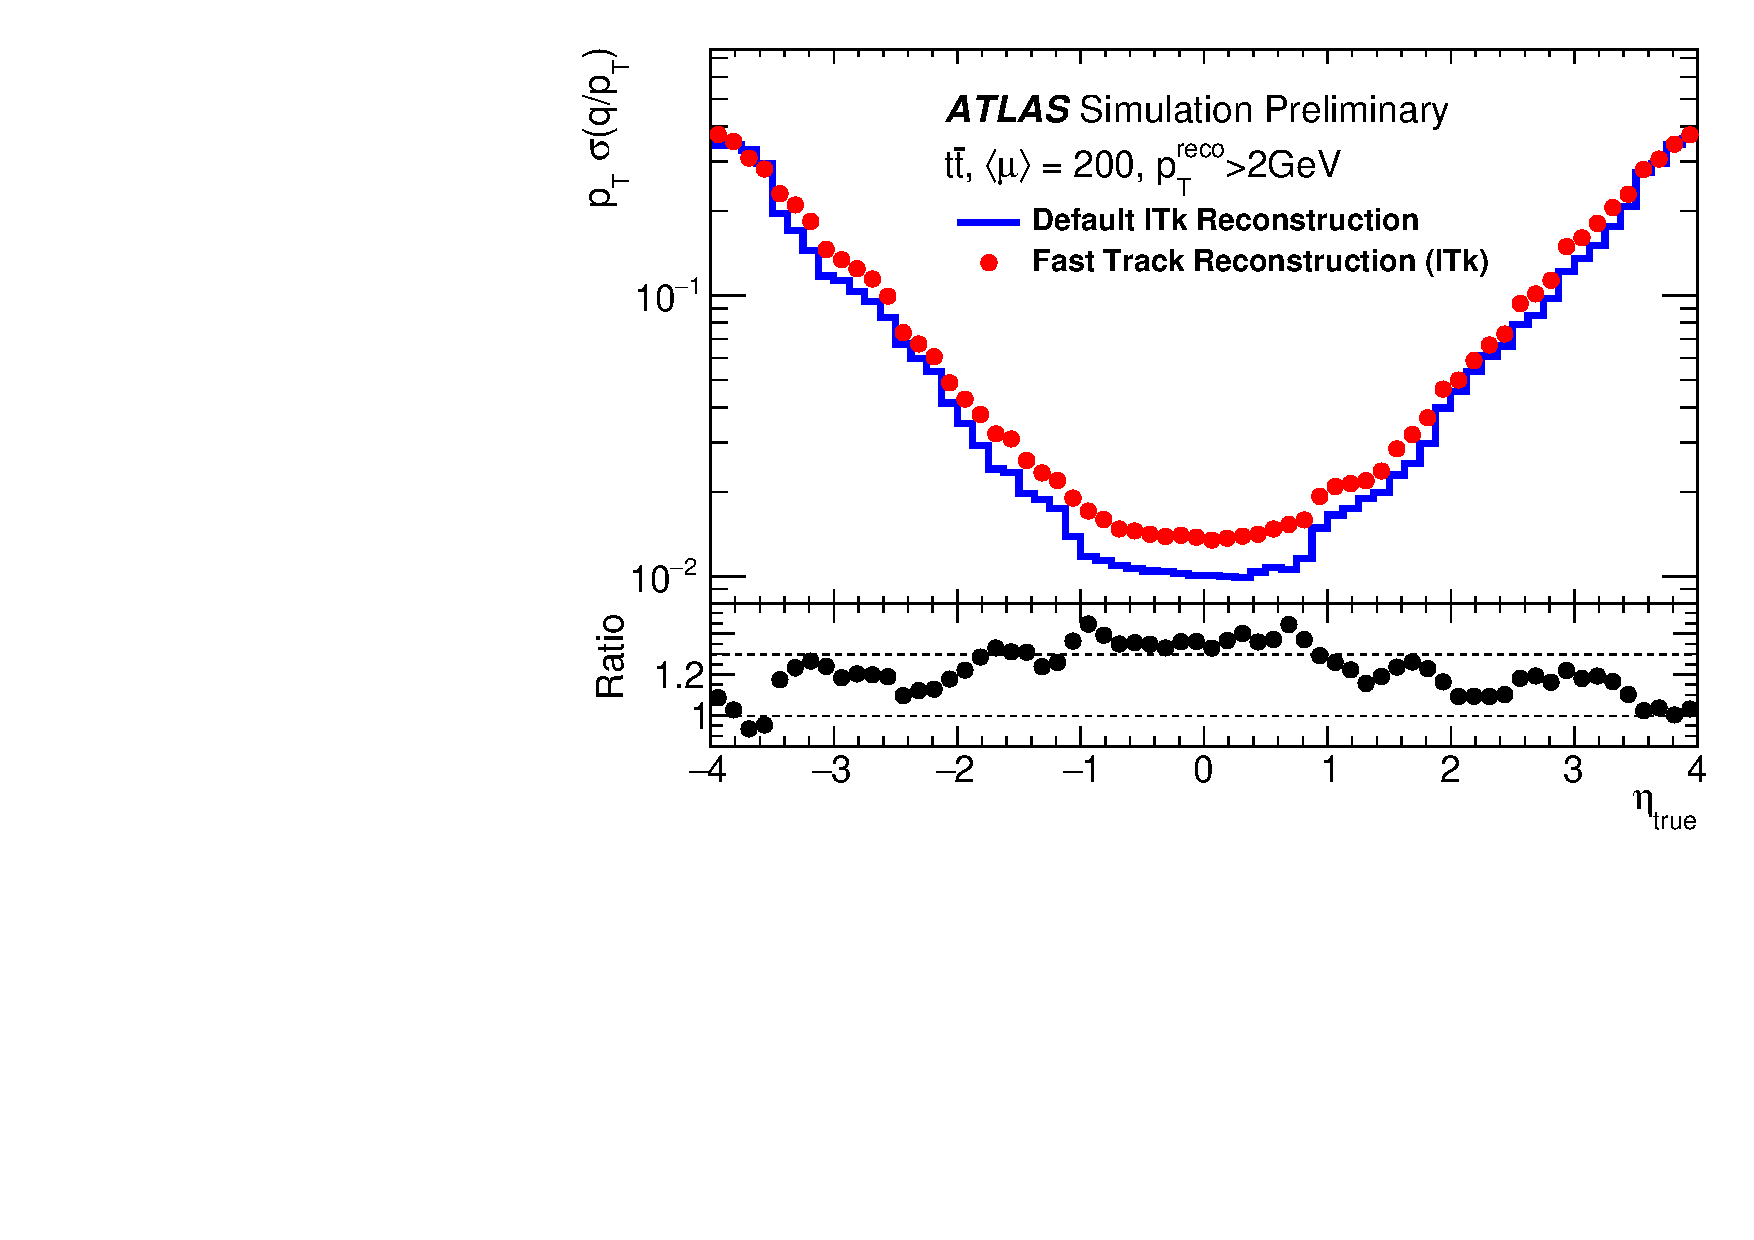
\includegraphics[width=0.50\textwidth]{figures/QoPEtaRatio}
  \caption{{\bf Left:} Tracking efficiency as a function of $\eta$ for the fast and the default ITk reconstruction. {\bf Right:} Relative transverse momentum $p_T$ as a function of $\eta_{true}$. Samples of $t\bar{t}$~events are used with $\langle\mu\rangle = 200$. A $p_T$ cut of 2~GeV is used for the generated particles, to avoid turn-on effects. The ratio is given by the efficiency for the fast reconstruction divided by the efficiency for the default reconstruction.}
  \label{fig:FastTrackingPerf}
\end{figure}

As expected because of the preliminary nature of this study, the fast ITk track reconstruction yields some loss in physics performance due to approximations made. Figure~\ref{fig:FastTrackingPerf} shows the loss in track reconstruction efficiency and in momentum resolution when comparing the fast and the default reconstruction on a sample of $t\bar{t}$~events with an average of 200 pile-up. A more detailed assessment of the tracking performance can be found in Reference~\cite{ATL-PHYS-PUB-2019-041}. This study demonstrates that it is possible to address the ITk track reconstruction problem for Phase-2 levels of pile-up using current tracking techniques on a classical CPU.

%%%%%%%%%%%%%%%%%%%%%%%%%%%%%%%%%%%%%%%%%%%%%%%%%%%%%%%%%%%%%%%%%%%%%%%

\subsection{The ATLAS Reconstruction Software Upgrade using ACTS}

The goal of the ATLAS Phase-2 software upgrade programme is not only to achieve the ultimate physics performance, but at the same time to modernise the software technology and to make best use of coming and future processing technologies. Technical performance improvements are expected in the area of event data model, data structures and data locality, in mathematical library optimisation and in the algorithms used for reconstruction.
%
\begin{comment}
\begin{figure}[htb!]
  \centering
  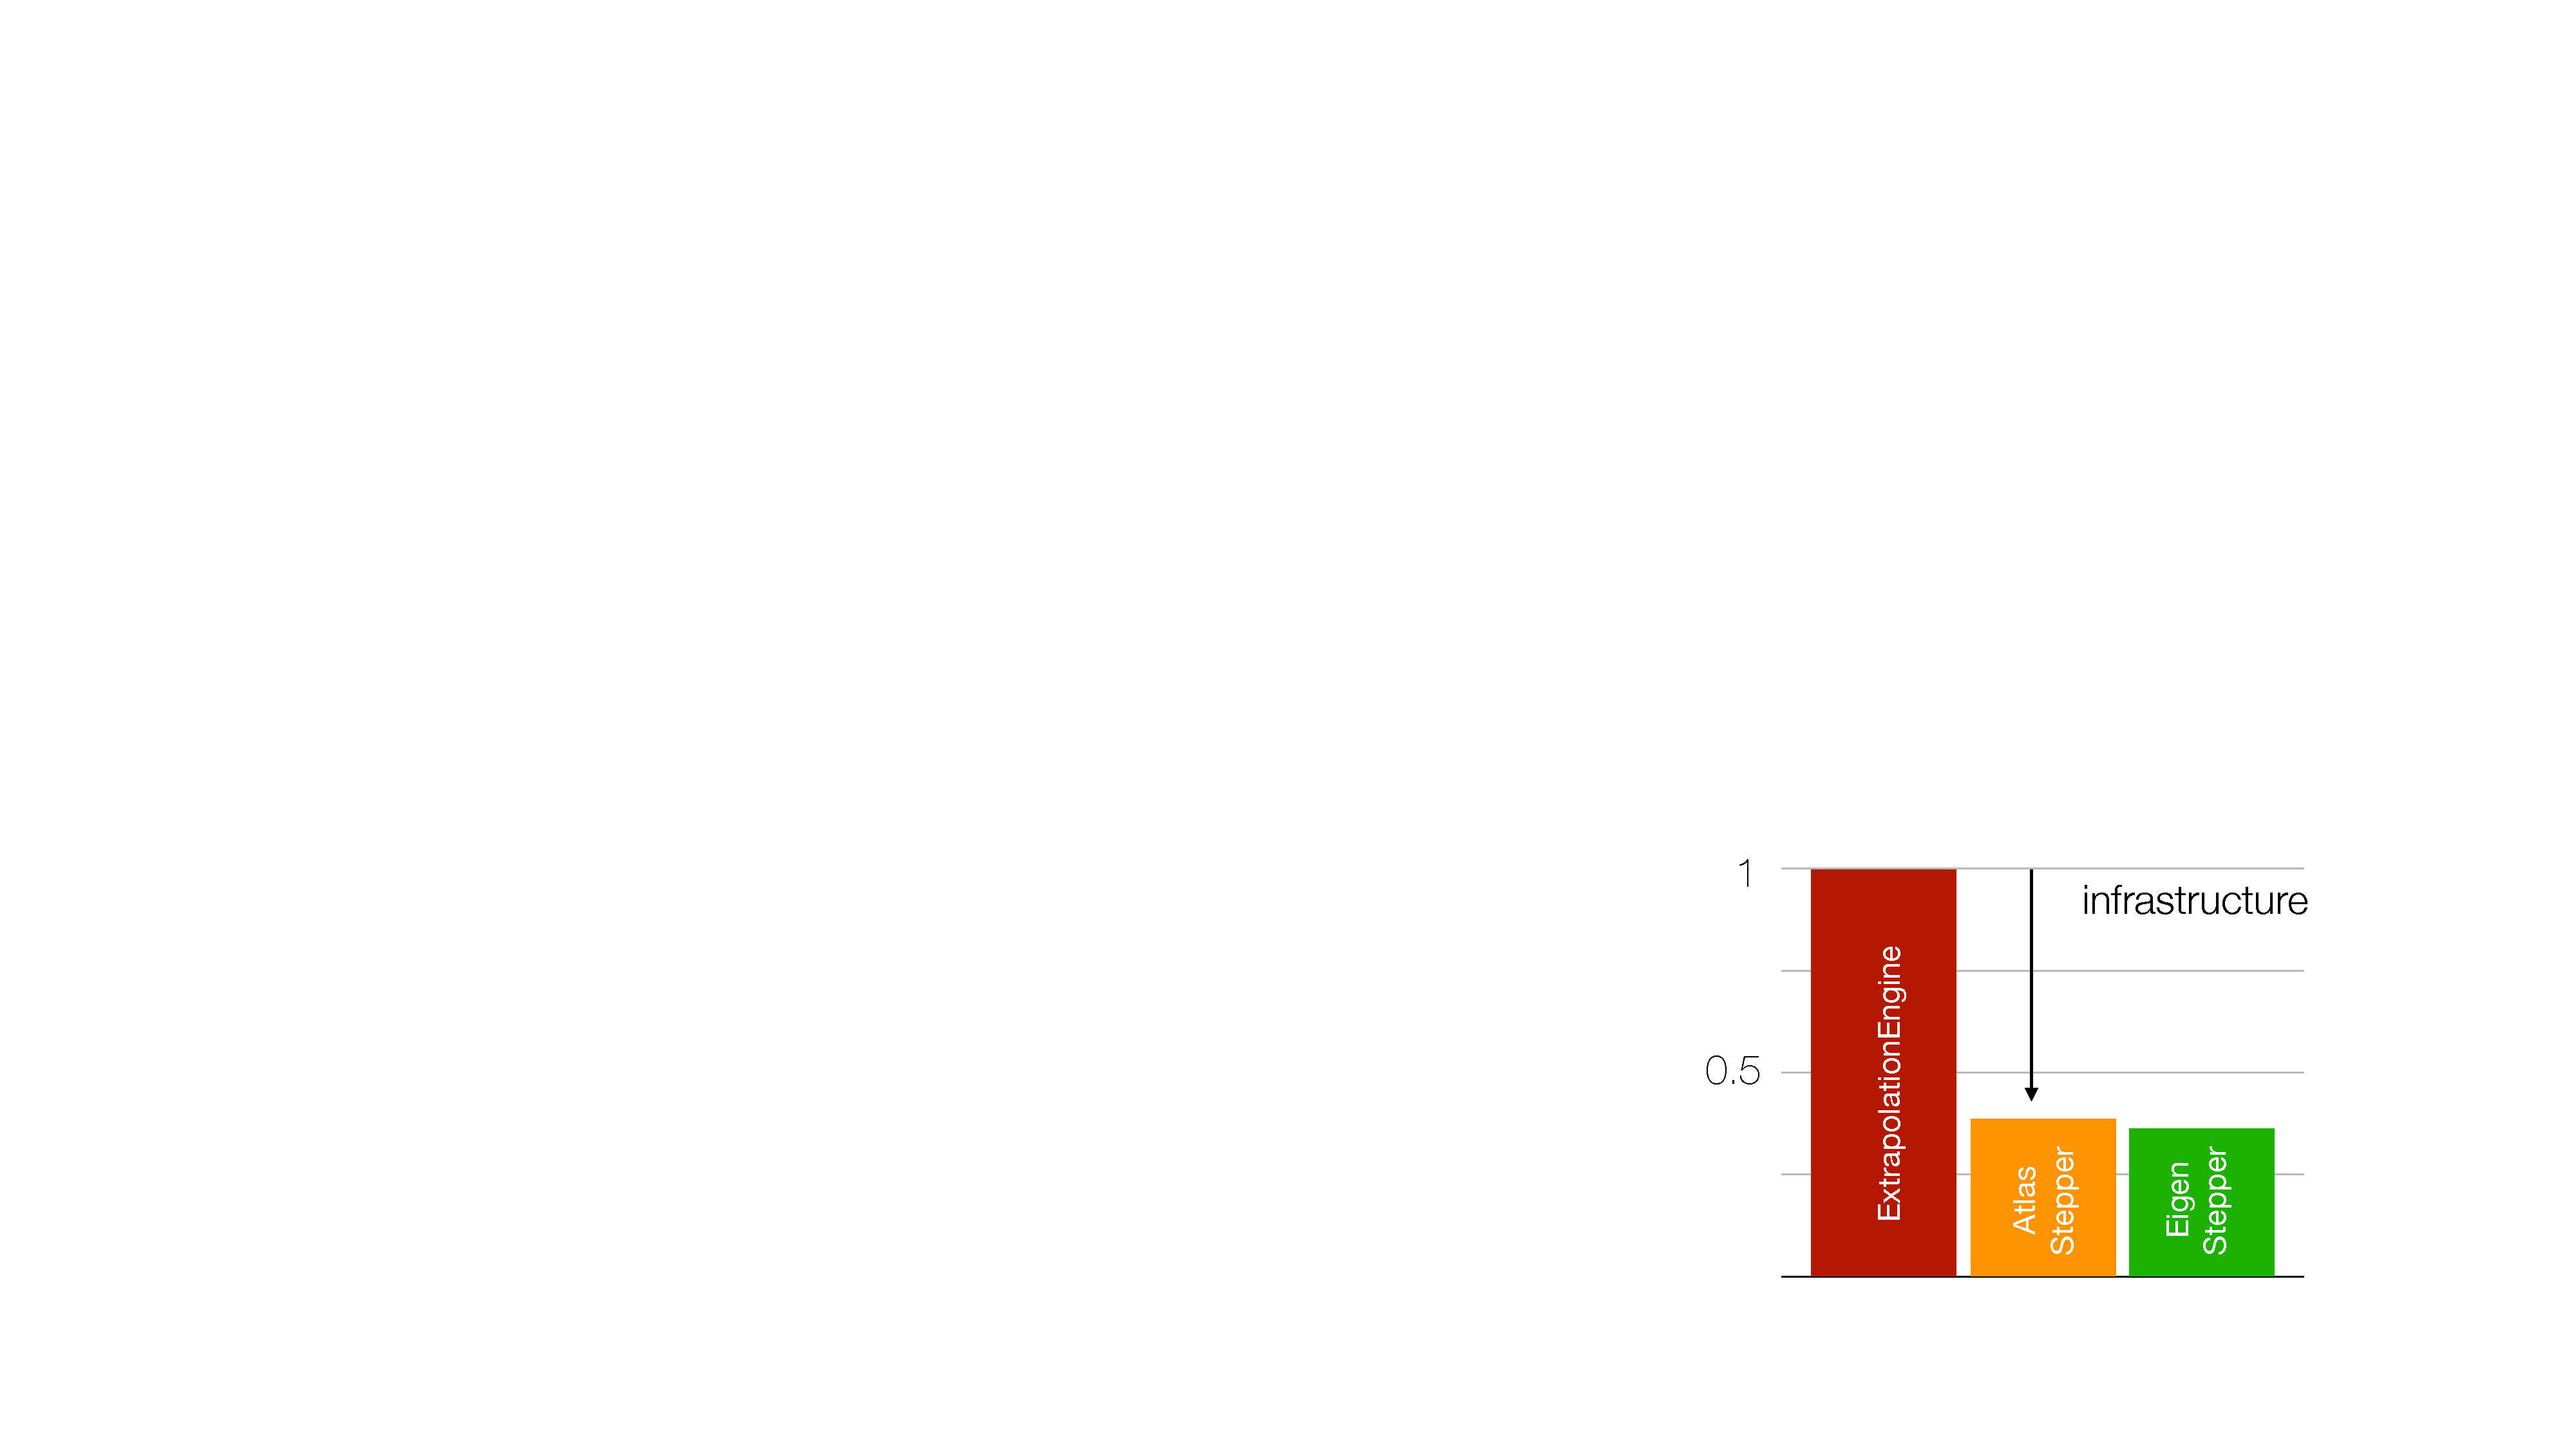
\includegraphics[width=0.40\textwidth]{figures/ACTSStepper}
  \caption{Relative timing comparison between two magnetic field stepping tools with the current ATLAS default extrapolation engine. Figure is taken from Reference~\cite{AndiCHEP2018}.}
  \label{fig:ACTSPerf}
\end{figure}
\end{comment}

ATLAS has launched the ACTS project~\cite{ACTS} as an open source tracking software project within the HEP community at large. The ACTS tracking software suite has been designed from the start for multi-threaded event processing and having data locality in mind. It significantly simplifies the technical overheads w.r.t. the current ATLAS tracking software and is aimed at a better utilisation of vector processing capabilities of modern CPUs. ATLAS is currently in the process of integrating the first functional components of the ACTS suite for the Run~3 event reconstruction. 
% Figure~\ref{fig:ACTSPerf} show an example for the technical performance improvements expected using ACTS compared to the current offline tracking software. The plot compares the relative speed for two of the the magnetic field integration stepper implemented in ACTS with the corresponding field integration using the ATLAS extrapolation engine. Figure is taken from Reference~\cite{AndiCHEP2018}.

Replacing the current suite of tracking tools use in the current Run~2/3 reconstruction with ACTS will result in significant CPU gains across the application, from the Inner Detector and Muon Spectrometer tracking, to all combined reconstruction using charged tracks. An important deliverable of the ACTS projects is a fast combinatorial Kalman filter, that will be used in the fast Silicon Track Finding to recover the full physics performance. The same Kalman filter will be used in the Ambiguity Resolution together with the Neural Network cluster splitting to recover from physics performance losses of the fast ITk track reconstruction prototype in the core of dense jets.
% Monte Carlo studies show that with this strategy the Ambiguity Resolution will only be applied to less than 5\% of the track candidates.
% The Bremsstrahlung option of the ACTS Kalman filter will used to recover inefficiencies for electron track in the fast Silicon Track Finding, adding a few \% to the total CPU budget for ITk reconstruction.

The Muon Spectrometer and combined muon reconstruction will benefit from the improved technical performance of the ACTS tracking tools. The new ACTS Gaussian Sum filter implementation is foreseen to replace the current software in the combined electron reconstruction and the ACTS extrapolation code will be used for the particle flow algorithm combining calorimeter and tracking information for jet finding and missing energy reconstruction. Primary vertex reconstruction, conversion finding, $tau$ reconstruction and $b$-tagging will be based on the ACTS vertexing package. The reconstruction of the Phase-2 High Granularity Timing Detector (HGTD) will use the ACTS software for associating timing hits to forward tracks.

%%%%%%%%%%%%%%%%%%%%%%%%%%%%%%%%%%%%%%%%%%%%%%%%%%%%%%%%%%%%%%%%%%%%%%%

\subsection{Optimising Reconstruction for Phase-2 Levels of Pile-up}

The physics performance of all object reconstruction and identification at Phase-2 needs to match and where possible exceed the current Run~2 performance, if ATLAS wants to reach its physics goals. All algorithms in the reconstruction chain need to be fully optimised for high pile-up, taking into account the CPU resource limitations. Technical software improvements, like the introduction of ACTS for the full reconstruction chain, are essential to meet the goals.

ATLAS is running an ambitious development programme for improved and novel algorithmic approaches for all detector and combined reconstruction aspects. Examples are optimised strategies for combined muon reconstruction that improve the acceptance for soft muons or handle more gracefully events with hadronic showers leaking into the Muon Spectrometer.

Calorimeter reconstruction is expected to not be affected by the high luminosity, both in terms of CPU time consumption and memory usage and both for data and Monte Carlo simulations.
This is due to the particular reconstruction algorithms for this detector system, which are described in detail in Ref. \cite{Aad:2016upy}. As for Run~1 and Run~2, they start from the whole (fixed size) list of individual signals and yield a stable average number of final signal objects (topological cell clusters), rather independent of the luminosity. 
While the existing calorimeter reconstruction algorithms are not expected to change significantly,
possible reconstruction performance improvements and computing resource reductions are under study. 
In particular, these include the formation and calibration of the topological cell clusters using machine learning techniques (see Reference~\cite{PERF-2014-07}).

New particle flow \cite{PERF-2015-09} objects will be introduced that support a more efficient extraction of overlapping and shared signals in complex Phase-2 events and thereby allow to extract efficiently an unambiguous event representation. Improved techniques for pile-up rejection will be developed for all combined reconstruction, exploiting the detailed particle flow information, the improved tracking performance with the ITk and the timing information from the HGTD in the forward. 

%%%%%%%%%%%%%%%%%%%%%%%%%%%%%%%%%%%%%%%%%%%%%%%%%%%%%%%%%%%%%%%%%%%%%%%

\subsection{Streamlining Reconstruction for Unconventional Signatures of New Physics}
\label{sec:reco-unconvsig}

One of the primary goals of the (HL-)LHC physics programme is the search for New Physics. Several models for New Physics give rise to experimental signatures involving meta-stable particles. A possible signature are charged particles decaying within the tracking system, leading to signatures of so-called disappearing tracks. Meta-stable heavy particles, as e.g. predicted in some R-parity violating SUSY models, may give rise to displaced production vertices for charged particles that tend to have large impact parameters and are only measured in the outer layers of the tracking system.

During Run~2 ATLAS was using a so-called pixel tracklet reconstruction step run after the primary track finding to identify candidates for disappearing tracks. A dedicated trigger stream was used to pre-select candidate events for CPU intensive reconstruction of tracks from displaced vertices. A significant fraction of the total CPU for data reconstruction was spend on the processing of the additional stream of selected displaced vertex candidate events, which also required significant additional data storage capacities. ATLAS aims to simplify the reconstruction strategy for such unconventional signatures for Phase-2. It is planned to integrated the pixel tracklets as a second track selection strategy in a unified single path Silicon Track Finding step, minimising the additional CPU resources needed. Because of the significant differences between the detector signatures of primary charged particles and those for displaced tracks, a second path of the Silicon Track Finding will be required. To limit the amount of CPU resources needed, this second path will only be applied to events pre-selected by dedicated trigger signatures.

Integrating the track reconstruction for unconventional signatures into the data processing chain will increase the CPU requirement for Tier-0, but the total amount of CPU required for reconstruction will be significantly reduced and the data processing model will be simplified, also reducing the amount of storage needed during Phase-2.

%%%%%%%%%%%%%%%%%%%%%%%%%%%%%%%%%%%%%%%%%%%%%%%%%%%%%%%%%%%%%%%%%%%%%%%

\subsection{Prospects for the technical Performance of the Phase-2 Reconstruction}

Two scenarios for the technical performance of the Phase-2 reconstruction were studied. The results of the current Run~2 based software for Phase-2 reconstruction are used as a baseline. Future improvements from the fast ITk reconstruction, the introduction of ACTS, the improvements in muon and calorimeter software, as well as in combined reconstruction, are expected to lead to significantly lower CPU resource requirements as a result of the Phase-2 reconstruction software upgrade programme.
%
\begin{table}[htb!]
  \caption{Prospects for CPU required in HS06~$\times$~seconds for reconstruction at different levels of average pile-up for Phase-2. Shown are the numbers for a $t\bar{t}$ Monte Carlo sample as measured for the current Run~2 based reconstruction software. In brackets the goals of the software upgrade programme are shown exploiting the Fast Track Reconstruction, ACTS and further technical and algorithmic optimisation of all aspects of the reconstruction software chain. Results for MC truth processing and framework overheads for I/O (etc.) are not included.}
  \label{tab:Phase2CPU}
  \centering
  \begin{tabular}{|c||c|c|c|c|c||c|} \hline
    \,\,\,\,\,$\langle\mu\rangle$\,\,\,\,\, & primary tracking & unconventional & calorimeter,      & combined       & monitoring & total reconstruction \\
                        &                  & signatures     & muon spectrometer & reconstruction &            &       \\ \hline
    140                 & 124 (35) & - (25)         & 157 (85)          & 51 (35)        & 70 (35)    & 402 (215)  \\
    200                 & 214 (50) & - (30)         & 176 (95)          & 94 (70)        & 100 (50)   & 584 (295) \\ \hline
    \end{tabular}
    % default is measured in 20.20 on ttbar
    % the assumption is that ACTS and technical updates with gain 30% in muon tracking, drop MuGirl
    % calo reco unchanged
    % 30% on egamma, jets, met. tau etc unchanged
\end{table}

Table~\ref{tab:Phase2CPU} summarises the technical CPU requirements for the baseline scenario using the current Run~2 based reconstruction software and, in brackets, when extrapolating the expected software and algorithmic improvements from the Phase-2 software upgrade programme. The evolved scenario includes the CPU for the reconstruction of unconventional signatures in the normal processing chain. The budget for offline monitoring on real data for Phase-2 is assumed to be 100 HS06~$\times$~seconds and 50 for the improved scenario, for running at 200 pile-up. At 140 pile-up 70 and 35 is assumed, respectively.

The software upgrades, if successful, may lead to more than a factor two speed improvement, compared to the current Run~2 software, also incorporating the processing of events for unconventional signatures. Track reconstruction will still account for a significant fraction of the overall reconstruction time, with a larger number of other reconstruction steps contributing at a similar level to the total CPU needed.

%%%%%%%%%%%%%%%%%%%%%%%%%%%%%%%%%%%%%%%%%%%%%%%%%%%%%%%%%%%%%%%%%%%%%%%

\subsection{Algorithm R\&D, Machine Learning and co-Processors}

The offline reconstruction will need to be adapted to the rapid evolution in software and processing technologies. Over the past years Machine Learning and other Data Science inspired techniques have been developed that promise to boost the physics performance for all aspects of event reconstruction. Techniques like similarity hashing, metric learning or graph networks are being investigated as alternatives~\cite{InstutitePascalTracking} to the classical track reconstruction techniques. For Phase-2 such novel techniques may be applied in the offline reconstruction or trigger context, also with the goal improve the technical CPU performance. It is therefore vital that ATLAS continues to further invest in such R\&D.

Most current and next generation HPC systems will provide the majority of their computing power in form of GPU co-processors. Online reconstruction for trigger processing can potentially benefit from deploying GPU co-processors in the trigger farm of the experiment. While all GPU co-processors offer large parallel processing capabilities, the model for programming those devices significantly differs from classical X86 processors. Supporting a heterogeneous set of co-processor technologies is therefore also a software development challenge. ATLAS is currently exploring different technologies like CUDA, OneAPI, Kokkos and alpaka for the integration of co-processors in its offline event processing framework ATHENA~\cite{ATHENA}. The aim is to develop tools for efficient offloading of algorithmic code onto different co-processors using the same code base and to minimise the need of vendor specific software development for the applications itself.

The model of using GPU co-processors for event reconstruction depends on the sharing of workloads in the application. Offloading of a few algorithmic kernels, that otherwise would require a large fraction of the overall CPU budget, is not possible for the ATLAS Phase-2 event reconstruction. As can be seen in Table~\ref{tab:Phase2CPU}, the improvements of the fast ITk track reconstruction will yield to a much more even distribution of CPU needed for the different algorithmic parts of the event reconstruction chain. Packages like ACTS and new ATLAS algorithmic code developed for Phase-2 are being designed from the start to better support parallel processing. Memory models required for efficient processing on GPU co-processors will also help improving data locality for X86 processing. Novel Machine Learning and Data Science inspired algorithmic approaches for event reconstruction are also evaluated for the ability to exploit GPU co-processors. The exact model for a more fine-grained offloading of algorithmic workloads onto co-processors is yet a subject of intensive R\&D. The ATLAS Phase-2 computing model extrapolations for offline reconstruction are therefore based on X86 processing and no assumptions are made on additional gains from particular co-processing and related software technologies.